\documentclass[12pt]{article}
 
\usepackage[margin=.75in]{geometry} 
\usepackage{amsmath,amsthm,amssymb}
\usepackage{bm}
\usepackage{enumitem}
\setenumerate{listparindent=\parindent}

\usepackage[english]{babel}
\usepackage[utf8]{inputenc}
\usepackage{amsmath,amssymb, amsthm}
\usepackage{graphicx}
\usepackage{amssymb}
\usepackage{verbatim}
\usepackage{gensymb}
\usepackage{bm}

\usepackage{tikz}
\usepackage{tkz-berge}
%\usepackage{graphics,graphicx}
%\usepackage{pstricks,pst-node,pst-tree}
\usepackage[colorinlistoftodos]{todonotes}
\usetikzlibrary{arrows,shapes,positioning}
%\usetikzlibrary{positioning,arrows}
 
 
\newcommand{\N}{\mathbb{N}}
\newcommand{\Z}{\mathbb{Z}}
\newcommand{\p}{\mathcal{P}_2(T)}
\newcommand{\Aut}{\textnormal{Aut}(P)}

 
\begin{document}
 
% --------------------------------------------------------------
%                         Start here
% --------------------------------------------------------------


\title{Math 172 - HW 2}
\author{Michael Knopf}
 
\maketitle

%%%%%%%%%%%%%%%%%%%%     1     %%%%%%%%%%%%%%%%%%%%%%%%

\begin{enumerate}[leftmargin=0cm,itemindent=.5cm,labelwidth=\itemindent,labelsep=0cm,align=left]

\item (VLW, 3B) Let the edges of $K_7$ be colored with red and blue colors.  Show that there are at least 4 subgraphs isomorphic to $K_3$ with all three edges having the same color.  Also show that equality is possible.

\begin{proof}

\ A subgraph isomorphic to $K_3$ is just a triangle formed in the vertices of $K_7$.  If not all edges in such a triangle are of the same color, call it a ``bad" triangle.  Also, if some edges $(a,b)$ and $(b,c)$ are of a different color, then say that they form a ``bad" angle.  Every bad triangle contains two edges of the same color and one of another color.  Thus a bad triangle contains exactly two bad angles.

Every vertex of $K_7$ is incident with $6$ edges.  By the pigeonhole principle, at least 3 of these are of the same color.  If it is incident with $k \in \{3,4,5,6\}$ edges of one color, then it is also incident with $6-k$ edges of the other color.  So it forms exactly $k \cdot (6-k)$ bad angles, since each of the $k$ edges forms a bad angle with each of the $6-k$ other edges.  Thus each vertex forms at most 9 bad angles (when $k = 3$), so $K_7$ contains at most 63 bad angles.

Since each bad triangle contributes $2$ bad angles, $K_7$ can contain at most $\lfloor \frac{63}{2} \rfloor = 31$ bad triangles.  Since $K_7$ contains $\binom{7}{3} = 35$ total triangles, there must be at least $35 - 31 = 4$ triangles where all edges are the same color.

In the graph below, there are exactly 4 triangles with all edges the same color: $(1,4,7)$, $(1,4,5)$, $(3,4,6)$, and $(2,5,6)$.
\begin{figure}[h]
\begin{center}
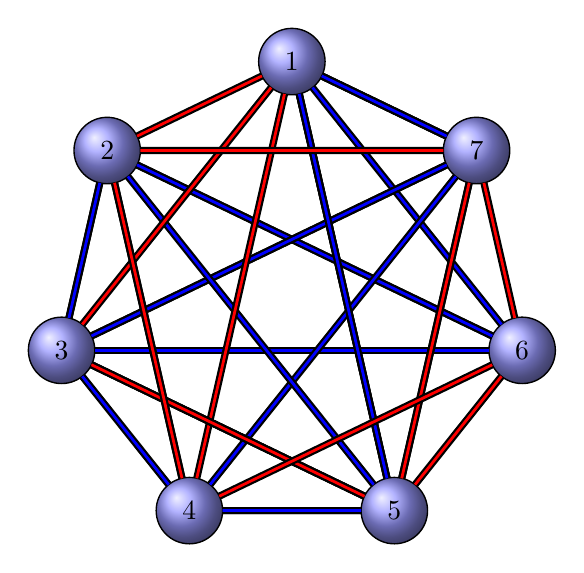
\begin{tikzpicture}[rotate = 90]
%\begin{scope}[rotate=90]
\renewcommand*{\VertexBallColor}{blue!40!white}
\GraphInit[vstyle=Shade]
\SetUpEdge[color=black,lw=1pt]
\tikzset{EdgeStyle/.style =
{thick,
double = blue,
double distance = 1pt}}
\SetGraphUnit{3}
\Vertices{circle}{1,2,3,4,5,6,7}
\Edges(1,5,1,7,1,6,2,6,3,2,3,7,3,4,7,1,5,4,5,2)
\SetUpEdge[color=black,lw=1pt]
\tikzset{EdgeStyle/.style =
{thick,
double = red,
double distance = 1pt}}
\Edges(1,2,4,1,3,5,6,7,5,3,5,7,2,4,6)
\end{tikzpicture}
\end{center}
\end{figure}

\begin{figure}[h]
\begin{center}
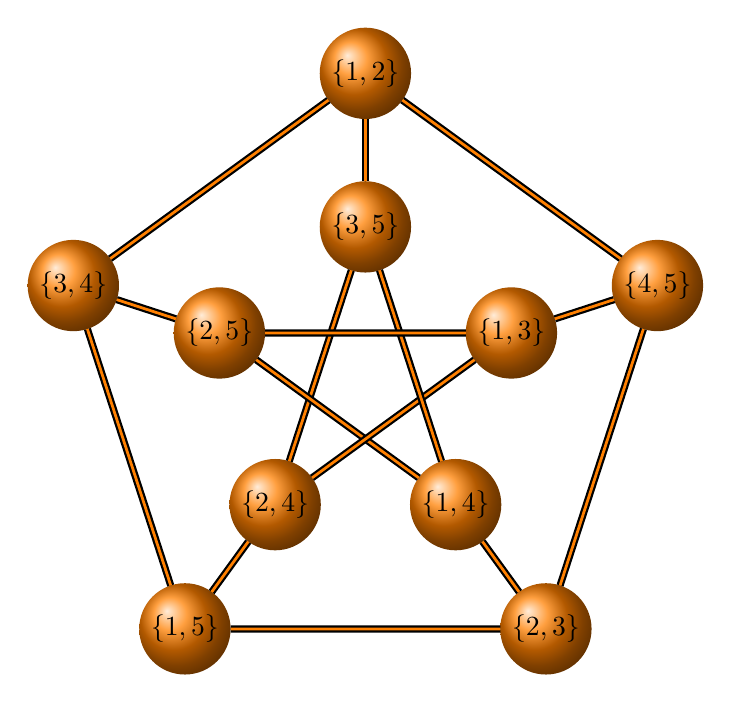
\begin{tikzpicture}[scale = 1.3, rotate=90]

  \newcommand{\aset}[2]{$\{#1,#2\}$}
  \GraphInit[vstyle=Art]
  \SetVertexNoLabel
  \SetUpVertex[MinSize=33pt]
  \SetUpEdge[color=black,lw=1pt]
  \tikzset{EdgeStyle/.style =
	{thick,
	double = orange,
	double distance = 1pt}}
  \grPetersen[RA=3,RB=1.5]
  \AssignVertexLabel{a}{\aset{1}{2},\aset{3}{4},\aset{1}{5},\aset{2}{3},\aset{4}{5}}
  \AssignVertexLabel{b}{\aset{3}{5},\aset{2}{5},\aset{2}{4},\aset{1}{4},\aset{1}{3}}

\end{tikzpicture}
\end{center}
\end{figure}

%\GraphInit[vstyle=Hasse]
%\begin{tikzpicture}
%  \pgfmathsetmacro{\theshift}{4/(1+sin(30))-2}
%  \begin{scope}[yshift=-\theshift cm]
%    \grTetrahedral[RA=4/(1+sin(30))]
%  \end{scope}
%  \draw (0,-2.5) node [fill=magenta!30!white,below]{$K_{4}$};
%  \pgfmathsetmacro{\theshift}{4/(1+sin(54))-2}
%  \begin{scope}[xshift=6cm,yshift=-\theshift cm,rotate=90]
%    \grComplete[RA=4/(1+sin(54))]{5}
%  \end{scope}
%  \draw (6,-2.5) node [fill=magenta!30!white,below]{$K_{5}$};
%  \begin{scope}[xshift=12cm]
%    \grComplete[RA=2/sin(60)]{7}
%  \end{scope}
%  \draw (12,-2.5) node [fill=magenta!30!white,below]{$K_{6}$};
%\end{tikzpicture}
%
%
%\begin{tikzpicture}
%  \SetVertexNormal[MinSize=12pt]
%  \tikzset{VertexStyle/.append style=
%    {inner sep=0pt,font=\footnotesize\sffamily}}
%  \begin{scope}[rotate=-90]
%    \grCirculant[RA=0.6,prefix=a]{5}{2}
%  \end{scope}
%  \begin{scope}[rotate=-18]
%    \grEmptyCycle[RA=1.5,prefix=b]{5}{2}
%  \end{scope}
%  \begin{scope}[rotate=18]
%    \grCycle[RA=2.5,prefix=c]{5}
%  \end{scope}
%  \EdgeIdentity{a}{b}{5} 
%  \EdgeIdentity{b}{c}{5}
%  {\tikzset{EdgeStyle/.append style = {blue,line width=3pt}}
%  \EdgeDoubleMod{b}{5}{0}{1}{a}{5}{2}{1}{5}}
%  {\tikzset{EdgeStyle/.append style = {green,line width=2pt}}
%  \EdgeDoubleMod{c}{5}{0}{1}{b}{5}{1}{1}{5}}
%\end{tikzpicture}


\end{proof}

\item Find all automorphisms of the Petersen Graph.

\begin{proof}

\ Let $P$ denote the Petersen graph.  Let $T = \{1,2,3,4,5\}$ and denote by $\p$ the set of all two element subsets of $T$.
We can label the vertices of $P$ using distinct two-element subsets of $T$ so that two vertices are adjacent if and only if their labeling sets are disjoint.  So there is a bijection $f:\p \rightarrow V(P)$ which induces a bijection between disjoint subsets of $\p$ and adjacent vertices of $P$.  Also, for any permutation $\sigma \in S_5$ we can define a permutation $\tau_\sigma$ on the vertices of $P$ by $\tau_\sigma = f \circ \sigma \ \circ f^{-1}$, where here we are actually considering $\sigma$ to be the map it induces on subsets of $\p$.

Let $\sigma \in S_5$ and $A,B \in \p$.  Then $A$ and $B$ are disjoint if and only if $\sigma(A)$ and $\sigma(B)$ are disjoint: if $x \in A \cap B$ then $\sigma(x) \in \sigma(A) \cap \sigma(B)$; and if $x \in \sigma(A) \cap \sigma(B)$ then $\sigma^{-1}(x) \in A \cap B$.  Thus, $x,y \in V(P)$ are adjacent if and only if $\tau_\sigma(x)$ and $\tau_\sigma(y)$ are as well.  Therefore, $\tau_\sigma \in \Aut$.  So we can define a map $\tau: S_5 \to \Aut$ by $\sigma \mapsto \tau_\sigma$.

It is not hard to see that $\tau$ is a homomorphism.  For any $\sigma_1, \sigma_2 \in S_5$, we have $\tau_{\sigma_1 \circ \sigma_2} = f \circ (\sigma_1 \circ \sigma_2) \circ f^{-1} = (f \circ \sigma_1 \circ f^{-1}) \circ (f \circ \sigma_2 \circ f^{-1}) = \tau_{\sigma_1} \circ \tau_{\sigma_2}$.

To see that $\tau$ is injective, assume $\sigma$ is not the identity permutation.  Then there are some distinct $a,b \in T$ such that $\sigma(a) = b$.  So for any other distinct element $c \in T$, $\sigma(\{a,c\}) = \{b,\sigma(c)\} \neq \{a,c\}$, therefore $\sigma \not \in ker(\tau)$.

Finally, we argue that $\tau$ is surjective.  Let $\varphi \in \Aut$.  Now, let $\sigma_1 \in S_5$ be any permutation such that $\tau_{\sigma_1} \circ \varphi$ fixes $f(\{1,2\})$ (we know such a permutation exists because all we require is that $\sigma_1$ map $f^{-1} \circ \varphi(f(\{1,2\}))$ to $\{1,2\}$, and there is always a permutation that maps any given two-element subset to $\{1,2\}$).

Next, choose a permutation $\sigma_2 \in S_5$ such that $\tau_{\sigma_2 \circ \sigma_1} \circ \varphi$ fixes both $f(\{1,2\})$ and $f(\{3,4\})$.  Since $\tau_{\sigma_1} \circ \varphi$ already fixes $f(\{1,2\})$, we need $\tau_{\sigma_2}$ to fix $f(\{1,2\})$ while sending $\tau_{\sigma_1} \circ f(\{3,4\})$ to $f(\{3,4\})$.  Because $\{1,2\}$ and $\{3,4\}$ are disjoint, though, such a $\sigma_2$ exists. ($\tau_{\sigma_1} \circ \varphi( f(\{3,4\})) = \{a,b\}$ where $\{a,b\} \cap \{1,2\} = \emptyset$.  So let $\sigma_2$ send $a$ to 3, $b$ to 4, and fix $1$ and $2$.)

Finally, choose $\sigma_3$ so that $\tau_{\sigma_3 \circ \sigma_2 \circ \sigma_1} \circ \varphi$ fixes $f(\{1,2\})$, $f(\{3,4\})$, and $f(\{3,5\})$.  If $\tau_{\sigma_2 \circ \sigma_1} \circ \varphi$ is the identity, then simply let $\sigma_3$ be the identity.  Otherwise, $\tau_{\sigma_2 \circ \sigma_1} \circ \varphi$ fixes $\{1,2\}$ and $\{3,4\}$, thus it must swap $3$ and $4$ while fixing $5$.  So let $\sigma_3$ swap 3 and 4 while fixing 1, 2, and 5, and we will have the desired result.  

Since the only remaining neighbor of $f(\{1,2\})$ is $f(\{4,5\})$, $\tau_{\sigma_3 \circ \sigma_2 \circ \sigma_1} \circ \varphi$ must fix this vertex as well, since the map must preserve the edge between it and $f(\{1,2\})$, but the only other vertices joined with $f(\{1,2\})$ are fixed.

If $\tau_{\sigma_3 \circ \sigma_2 \circ \sigma_1} \circ \varphi$ is the identity, then let $\sigma_4$ be the identity.  Otherwise, consider a vertex we have not already shown to be fixed - for instance, $f(\{2,5\})$.  This must go to a neighbor of $f(\{3,4\})$.  It cannot go to $f(\{1,2\})$, since this is fixed.  So the only option is to swap it with $f(\{1,5\})$.  This will mean that $f(\{1,3\})$ must swap with $f(\{2,3\})$ and $f(\{2,4\})$ must swap with $f(\{1,4\})$.  In fact, if any of these swaps are made then all of them must be.  So the resulting arrangement (shown below) is the only possible one if the composition is not the identity.  If this is the case, then let $\sigma_4$ swap $1$ and $2$ but fix everything else.

\begin{figure}[h]
\begin{center}
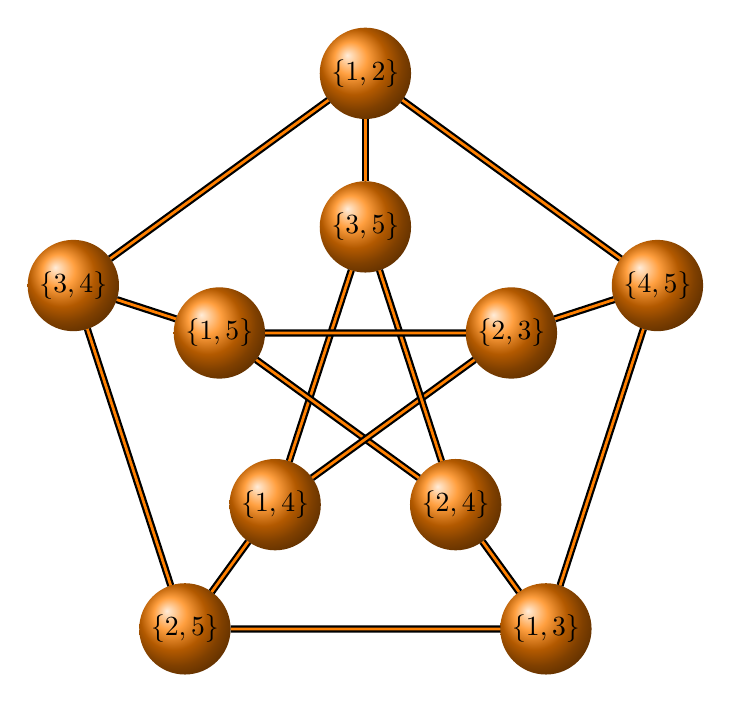
\begin{tikzpicture}[scale = 1.3, rotate=90]

  \newcommand{\aset}[2]{$\{#1,#2\}$}
  \GraphInit[vstyle=Art]
  \SetVertexNoLabel
  \SetUpVertex[MinSize=33pt]
  \SetUpEdge[color=black,lw=1pt]
  \tikzset{EdgeStyle/.style =
	{thick,
	double = orange,
	double distance = 1pt}}
  \grPetersen[RA=3,RB=1.5]
  \AssignVertexLabel{a}{\aset{1}{2},\aset{3}{4},\aset{2}{5},\aset{1}{3},\aset{4}{5}}
  \AssignVertexLabel{b}{\aset{3}{5},\aset{1}{5},\aset{1}{4},\aset{2}{4},\aset{2}{3}}

\end{tikzpicture}
\end{center}
\end{figure}



In either case, $\tau_{\sigma_4 \circ \sigma_3 \circ \sigma_2 \circ \sigma_1} \circ \varphi$ is the identity.  Thus $\varphi = (\tau_{\sigma_4 \circ \sigma_3 \circ \sigma_2 \circ \sigma_1})^{-1} = \tau_{(\sigma_4 \circ \sigma_3 \circ \sigma_2 \circ \sigma_1)^{-1}}$, so $\tau$ is surjective.  Therefore, the automorphism group of the Petersen Graph is isomorphic to $S_5$, and thus has $5! = 120$ elements.

\end{proof}

\item Fix positive integers $n$ and $k$, and let $S = [n]$.  Find the number of $k$-tuples $(T_1, T_2, \dots, T_k)$ of subsets $T_i$ of $S$ such that (a) the $T_i$ are pairwise disjoint; (b) $T_1 \cup T_2 \cup \cdots \cup T_k = S$.

\begin{proof}

(a) For each element of $[n]$, we have $k+1$ choices.  We may choose any of the $k$ sets to put it in, or put it in none of the sets.  This process will create $k$ subsets, which are pairwise disjoint because each element has been placed in at most one set.

If we do this process in two different ways, then there is some element $x \in [n]$ which was placed in some $T_j$ in one process, but not placed in $T_j$ in the other.  So the resulting $k$-tuples will differ in the $j$th position.

Given any $k$-tuple, it could have been created by this process: for each $x \in [n]$, place $x$ in $T_j$ if $x$ is in $T_j$.  If $x$ is not in any of the sets in the tuple, do not put it in any of the sets.

Thus we have created a bijection from the set of such $k$-tuples to the number of ways to do something $n$ times which can be done in $k+1$ different ways.  So there are $(k+1)^n$ such tuples.

(b) For each $i \in [n]$, choose a nonempty subset $S$ of $[k]$.  If $j \in S$, then place $i$ in $T_j$ (if $S$ contains multiple elements, put $i$ in all of the corresponding $T_j$s).

The resulting tuple will have the property $T_1 \cup T_2 \cup \cdots \cup T_k = S$ because each $i \in [n]$ was placed in at least one $T_j$, since we did not allow the empty set when choosing subsets of $[k]$.

If the process is done in two different ways, then there is some $i \in [n]$ for which $i$ was placed in $T_j$ during one process but not during the other.  Thus the resulting tuples will differ in their $j$th position.  Also, any such $k$-tuple can be created by this process.  If $i \in T_{i_1}, \dots, T_{i_l}$, then choose the subset $\{i_1, \dots , i_l \} \subseteq [k]$.

Thus we have created a bijection between the set of such $k$-tuples and the set of ways to choose a nonempty subset of $[k]$ $n$ times.  There are $(2^k - 1)^n$ ways to do this, because there are $2^k - 1$ nonempty subsets of $[k]$.

\end{proof}

\item Give a good definition of ``isomorphism" for simple \emph{directed} graphs (in terms of $V(G)$ and $E(G)$).  Count the number of isomorphic labeled and unlabeled directed trees on 5 vertices.

\begin{proof}

\ A directed graph $G$ is a set of vertices $V(G)$ along with a set of edges $E(G) \subseteq V(G)^2$.  A map $f: G \rightarrow H$ is an isomorphism if $f$ is a bijection such that $(x,y) \in E(G)$ if and only if $(f(x),f(y)) \in E(H)$.  For this problem, we are considering only simple directed graphs in which if $(a,b) \in E(G)$ then $(b,a) \not \in E(G)$.

Graphs (both directed and undirected) can be characterized by their isomorphism types.  Two labeled graphs are considered equivalent as unlabeled graphs if and only if they are isomorphic.

One unlabeled, undirected tree on $n$ vertices can be used to form another by removing one edge to create two disconnected components, then drawing a new edge that reconnects these components.  This process always creates a new tree, therefore any iteration of this process, applied to some tree on $n$ vertices, results in another tree on $n$ vertices.  Conversely, \emph{every} tree on $n$ vertices can be generated from a single one by applying this process.

If we take any of the trees below and apply this process once, removing an edge then adding a new one to connect the disconnected components, we obtain another of the trees below.  Since any tree can be created by this process, and this set of trees is closed under this process, every unlabled, undirected tree on $5$ vertices is one of these three.

\begin{figure}[h!]
%\caption{All unlabled, undirected trees on 5 vertices}
\begin{center}
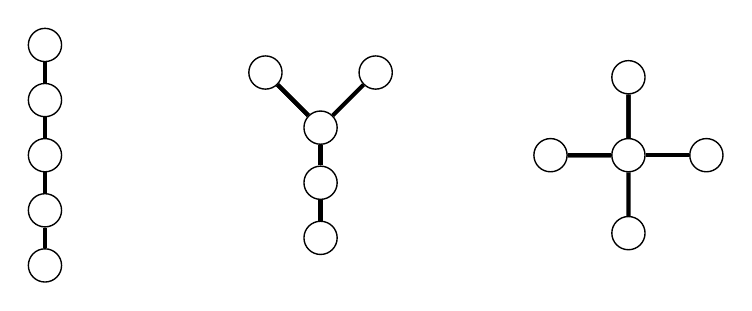
\begin{tikzpicture}[scale = .7]
\SetGraphUnit{1}
\GraphInit[vstyle=Hasse]
%\tikzset{EdgeStyle/.style = {->}}
\begin{scope}[rotate = 90]
\renewcommand{\VertexInnerSep}{0pt}
\Vertices{line}{A,B,C,D,E}
\SetUpEdge[lw=1.5pt]
\Edges(A,B,C,D,E)
\end{scope}

\begin{scope}[xshift=5 cm, yshift = .5cm, rotate = 90]
\Vertices{line}{A,B,C}
\NOEA(C){D}
\SOEA(C){E}
\SetUpEdge[lw=1.5pt]
\Edges(A,B,C,D,C,E)
\end{scope}

\begin{scope}[xshift=12 cm, yshift = 2cm, rotate = 90]
\SetGraphUnit{2}
\Vertices{square}{A,B,C,D}
\coordinate (E) at (intersection of A--C and B--D);
\Vertex[Node]{E}
\SetUpEdge[lw=1.5pt]
\Edges(A,E,B,E,C,E,D)
\end{scope}
\end{tikzpicture}

\end{center}
\end{figure}

To count the number of directed graphs on 5 vertices, we must sum the number of unique ways to give direction to these graphs.

The first tree yields $2^4 - 6 = 10$ directed trees, since we have $2$ choices for each of the $4$ edges, but the assignments wich are not symmetric across the middle vertex have been counted twice (there are 6 of these symmetric pairs, since there are $2^2$ symmetric assignments).

The second tree yields $2^2 \cdot 3 = 12$ directed trees: choose the direction of the bottom two edges, then choose whether the top two edges both point upwards, both point downwards, or point opposite directions (2 assignments result in them pointing in opposite directions, but these can be obtained from each other by reflection).

The last tree yields 5 directed trees.  All that matters is the number of out degrees of the middle vertex, which can be $0, 1, 2, 3$ or $4$.

Therefore, there are $10 + 12 + 5 = 27$ directed trees on $5$ vertices.

%To count the number of labled directed trees on 5 vertices, we can multiply the number of unique labelings of each of the three trees above by the number of unique ways to assign direction to it, then sum these.

For each of the nonsymmetric directed trees that form a line, there are $5!$ labelings, since symmetric labelings still produce unique labeled graphs.  For the symmetric directed trees of this form, there are $\dfrac{5!}{2}$ labelings, because of the one symmetry.  Thus there are $6 \cdot 5! + 4 \cdot \dfrac{5!}{2} = 960$ labeled directed trees of this form.

%The second trees yields $\dfrac{5!}{2} = 60$ labled trees for each directed tree, since every one of the $5!$ assignements is the same only as the one obtained by reflection.  So there are $\dfrac{5!}{2} \cdot 12 = 720$ labeled directed trees of this form.

For the claw shaped tree, each of the directed trees where the top two edges point the same direction have $2$ identical labelings, so this form contributes $(2^2 \cdot 2) \cdot \dfrac{5!}{2} = 480$.  For the trees where the top edges point different directions, all possible labelings are unique.  So these also contribute $2^2 \cdot 5! = 480$ trees.  Thus there are $960$ labeled directed trees of this form.

For the third tree, in the shape of a star, the directed trees where all directions point outwards or all directions point inwards are dependent only on the label of the center vertex.  So there are $5$ of each, thus these contribute 10.  For the star where the center vertex has outward degree of 2, there are $\dfrac{5!}{2^2} = 30$, because identical assignments are obtained by permuting the 2 outward legs and the 2 inward legs.  For the stars with outward degree 1 or 3, there are $\dfrac{5!}{3!} = 20$ labelings, since we may permute the labels of three legs which have the same direction.  So there are $2 \cdot 5 + 30 + 2 \cdot 20 = 80$ labeled directed trees of this form.

Thus there are $960 + 960 + 80 = 2000$ labeled directed trees on 5 vertices.

\end{proof}

\item Prove that a graph is $\emph{biparte}$ (this is a graph where the vertices can be written as a disjoint union $A\cup B$ such that the edges only go \textbf{between} $A$ and $B$, and never, say, between two vertices in $A$ or two vertices in $B$) if and only if there is no subgraph of form $C_n$, where $n$ is odd.

\begin{proof}

\ Suppose a graph $G$ is biparte, so that $V(G) = A \cup B$, and assume $C_n$ is a subgraph of $G$ for some $n$.  Let $V(C_n) = \{ v_0, \dots , v_{n-1} \}$ such that $(v_i, v_{i+1 \pmod{n}}) \in E(G)$ for all $i$.  Since $G$ is biparte, $v_i \in A$ if and only if $v_{i+1 \pmod{n}} \in B$, since these vertices are joined by an edge.  WLOG assume $v_0 \in A$.  Then by inductive application of the fact we have just derived, any even-indexed vertex is in $A$.  Thus, if $n$ is odd, then $n-1$ is even, so $v_{n-1} \in A$, so $v_0 = v_{(n-1) + 1 \pmod{n}} \in B$, a contradiction.  Therefore, $n$ is not odd.

Now, assume that $G$ has no subgraphs isomorphic to $C_n$ for odd $n$.  Let $H_1, \dots, H_k$ be the connected components of $G$.  For some $i$, let $v \in V(H_i)$.  Let $A_{H_i}$ be the vertices of $H_i$ for which the shortest path to $v$ is of even length, and let $B_{H_i}$ be those for which the shortest path to $v$ is of odd length.  Then $A_{H_i}$ and $B_{H_i}$ form a disjoint union of $H_i$.

Suppose $x,y \in H_i$ are adjacent.  Let $s$ and $t$ be the lengths of the shortest paths from $v$ to $x$ and $y$, respectively.  Then we may use these paths to make a path from $v$ to $x$ to $y$ and back to $v$, where the path from $x$ to $y$ has length 1.  Thus this whole path has length $s + t + 1$.

If the path from $y$ to $v$ retraverses the path from $v$ to $x$, then its length is $s+1$, thus the lengths of the shortest paths from $v$ to $x$ and from $v$ to $y$ have different parity.  So assume this is not the case.  Then the path from $y$ back to $v$ does not touch any vertex along the path from $v$ to $x$ (otherwise a shorter path would be made by retraversing that path completely).  Thus the complete path forms a subgraph isomorphic to $C_n$ (which is a path of length $n$), and by assumption $n$ must be even.  So the total length of the path $s + t + 1$ is even, so $s + t$ is odd.  Therefore, $s$ and $t$ have different parity in all cases.  So $x$ and $y$ come from different choices of $A_{H_i}$ and $B_{H_i}$.

Thus $A = \bigcup\limits_{i=1}^k A_{H_i}$ and $B = \bigcup\limits_{i=1}^k B_{H_i}$ form a partition of $G$ which satisfies the necessary conditions, so $G$ is biparte.
\end{proof}

\item $G$ is Eulerian if and only if the number of vertices with odd degree is 0 or 2.

\begin{proof}

\ Suppose $G$ is Eulerian, and let $v \in V(G)$ be a vertex that is not the first or last in the walk.  Then the edges incident with $v$ can be grouped into pairs - those entering $v$ in the walk and those leaving $v$.  Thus $v$ has even degree.  The total number of vertices in $G$ with odd degree must be even, so if the walk is closed then its starting vertex has even degree, thus there are 0 vertices with odd degree.  Otherwise, if the walk is open and WLOG its starting vertex has odd degree, then its ending vertex has odd degree as well, thus there are 2 vertices with odd degree.

Now suppose there are 0 or 2 vertices with odd degree, and induct on the number of vertices $n$ of $G$.  If $n=0$ or $n=1$, the result is vacuous.  If $n=2$, the result is clear.  So suppose any graph with $n$ vertices is Eulerian, and that $G$ has $n+1$ vertices for some $n > 2$.

Since $n > 2$, there is some vertex $v$ with even degree.  Group the edges incident with $v$ into pairs $(w_{i,1},v), (w_{i,2},v)$, and consider a new graph $H$ constructed by removing each of these edges and replacing them with a new edge $(w_{i,1}, w_{i,2})$ connecting the vertices from each pair that were connected to $v$.  Since each of these vertices has gained and lost an edge, its degree remains the same.  So by the inductive hypothesis, $H$ has a Eulerian path.  Since $(w_{i,1}, w_{i,2})$ is an edge in $H$, the path must contain a step from $w_{i,1}$ to $w_{i,2}$.  Insert $v$ in between these vertices in the path to create a Eulerian path on $G$.

\end{proof}

\item This homework was definitely easier than the last one.  \# 4 was probably the hardest problem because there are so many different cases to consider, so it is easy to make a mistake.  It is one of those problems that is difficult because it seems easy, so you trust your first instinct too much.  The Petersen Graph would definitely have been impossible if I hadn't seen the proof before.  Fun problems overall.

\end{enumerate}
\end{document}



















